% !TeX root = ../thuthesis-example.tex

\chapter{引言}

触摸交互是自然人机交互的重要组成部分,是人主动控制手指触摸交互表面,通过点击、长按、滑动等手势向计算机输入信息的方式。电容触摸屏作为触摸交互的主要载体已问世数十年,触摸交互技术得到了长足的发展,然而,触摸交互仍有改进空间,包括更强的普适性、更高的响应性和更准确的有意性判断。改进触摸交互的一条技术路线是充分利用触摸运动的规律,从原理的角度发掘改进触摸交互的机会。本章首先介绍触摸交互在人机交互领域的重要性和待改进方向,随后通过文献综述总结已有触摸交互技术及其不足,接下来简述本文提出的触摸运动模型及其研究内容,最后介绍论文组织结构。

\section{选题背景及意义}

\subsection{触摸交互的重要性}

目前,触摸交互是最重要的人机交互方式之一。2021年,手机、平板电脑等触摸屏设备的全球出货量达到15.1亿台,而笔记本、台式机等基于键鼠交互的设备的全球出货量为3.6亿台\cite{alsop2020shipment},其规模仅为触摸屏设备的23.8\%。相比于键鼠交互,触摸交互具有便捷、易学、自然等优势,使其适用于包括老人、儿童在内的更广泛用户群体。

【图:smartphone=1350; tablet=160; laptop=280; desktop=80】

在未来,触摸交互仍将是重要的研究课题。人机交互研究者普遍认为,头戴式混合现实设备(简称MR头盔,代表性产品是微软的Hololens2)是最有可能取代手机的下一代智能终端。MR头盔利用深度摄像头扫描物理环境,将虚拟元素叠加渲染在物理实体之上。如图\ref{fig:MR_touch_envision}所示,MR头盔中一种有前景的交互方式是将虚拟的用户界面渲染在无源表面上(如桌面、墙面),支持用户通过触摸与用户界面进行交互[xx]。触摸交互将摆脱触摸屏表面的限制,用户获得在任意表面上触摸交互的能力。与目前MR头盔中流行的空中手势交互相比,触摸交互为用户提供了触觉反馈和物理支撑,给交互的确认感[xx]、输入精度[xx]和抗疲劳性[xx]带来诸多好处。然而,目前MR头盔中的触摸交互技术尚未成熟,仍然值得进一步研究。

\begin{figure}
	\centering
	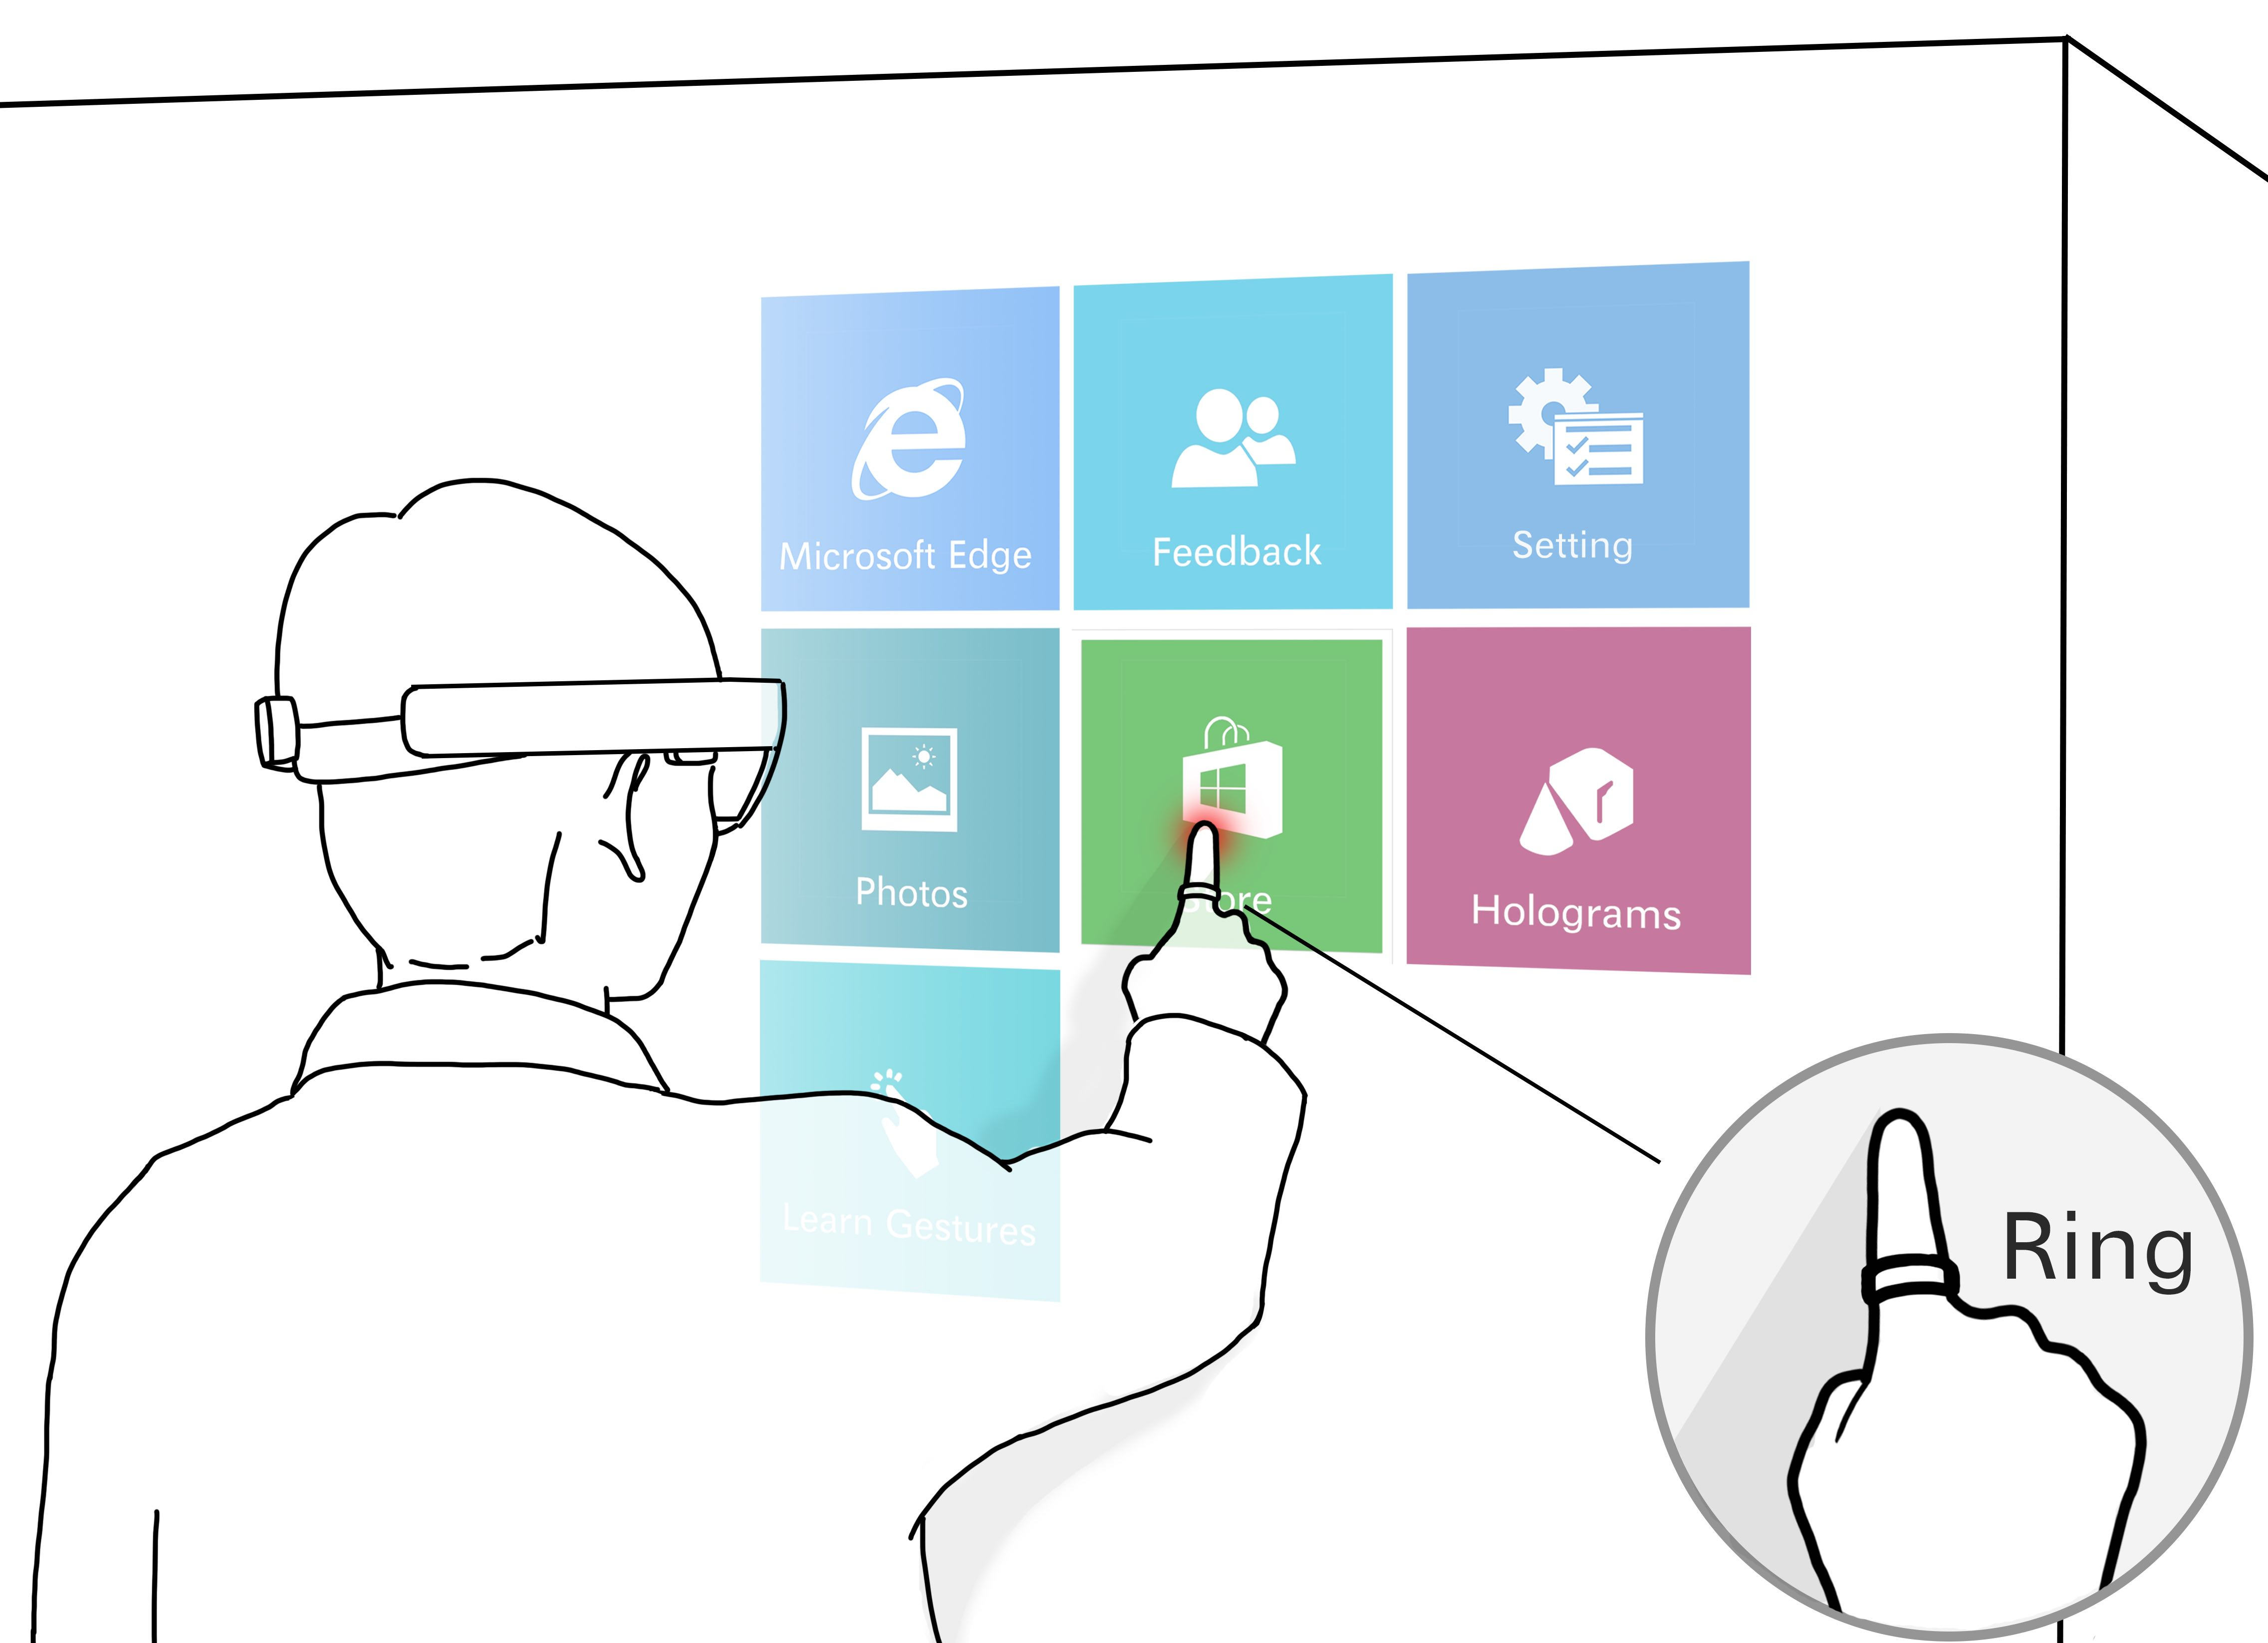
\includegraphics[width=0.8\linewidth]{MR_touch_envision.jpg}
	\caption*{介绍}
	\caption{名称}
	\label{fig:MR_touch_envision}
\end{figure}


\subsection{触摸交互的改进方向}

尽管触摸屏技术已经问世数十年,技术得到了长足的发展,但触摸交互仍有值得改进的地方,分别体现在普适性、响应性和有意性三个方面。

\textbf{(1)普适性}:普适计算是一个强调和环境融为一体的计算概念,主张计算设备朝小型化、可穿戴的方向发展,直至消失在人们的视线当中,人们能在任何时间、地点,以任何方式与与数字世界交互。在人机交互往普适计算发展的过程中,触摸屏等专用输入设备可能是第一批消失的,此时如何支持触摸交互是值得研究的问题。例如,上一小节中所述的基于MR头盔的触摸交互技术是增强触摸普适性的一个实例。

\textbf{(2)响应性}:人对触摸交互响应性的感官需求极高,在点击触摸任务中,人能察觉到低至10毫秒的端到端延迟,并对高于100毫秒的延迟感到极度厌烦[xx]。然而,目前智能手机触摸屏的延迟普遍在50毫秒以上,未能给用户提供极致的用户体验。一种容易察觉到延迟的方法是快速的拖拽任务,例如,在手机中长按APP图标并快速移动。尽管目前的触摸屏延迟在多数任务下不会让用户感到厌烦,但如果要将用户体验提升到最高水平,就需要将触摸交互的延迟降低到10毫秒以内,让用户无法察觉延迟的存在。

\textbf{(3)意图性}:自然动作交互是人机交互的发展趋势,其特点是有意动作和无意动作混杂,给交互的意图识别带来困难。例如,在目前的触摸屏十指打字中,用户必须将手悬空,久而久之会导致疲劳的问题,这种要求用户故意悬空手部以防止误触的交互方式是不自然的,应该开发一款强力的防误触算法,允许用户在打字的间隙将手指休息在触摸屏上(而不会引发误触);又例如,在上一小节所述的基于MR头盔的触摸交互模态中,用户既可以在普通的桌子上触摸交互,也可能仅仅是将手休息在桌子上,在此场景下的触摸交互技术需要发展出识别用户触摸是否具有交互意图的能力。

改进触摸交互的一条技术路径是充分利用触摸的运动规律,即总结触摸前后手指的位移、速度和加速度特征,建立触摸的运动模型。触摸的运动模型将有利于提高触摸交互的普适性、响应性和有意性,这是因为:(1)基于视觉方法的运动传感是普适计算场景下容易获得的传感能力;(2)触摸运动模型可利用手指触摸表面前的传感信号拟合触摸的运动方程,从而以低延迟、甚至负延迟识别触摸事件;(3)触摸运动方程中的参数将能作为判断触摸有意性的有效特征。

\section{研究现状}

\subsection{电容触摸屏}

很准确、常用,但在普适性、响应性和有意性上存在弊端。

\subsection{基于运动传感的触摸感知技术}

位置识别可以做到很准,但是触摸瞬间的感知是难点。

MR头盔中一种直观的感知触摸事件的方法,是利用MR头盔的前置摄像头来观察用户的手指是否接触到交互表面。然而, 基于视觉的方法在触摸感知方面存在两大内在缺点:首先,由于MR头盔的摄像头是从手背的方向观察手指运动的,手指与交互平面的接触点时常被遮挡,因此很难准确、低延迟地识别触摸事件;第二,基于手型恢复的视觉方法往往会消耗大量的计算资源,导致系统延迟过大,影响用户体验。出于以上原因,此前最先进的利用Hololens识别任意物体表面触摸事件的工作中,实验表面存在3.5\%的未识别点击和19.0\%的误触[xx],系统延迟达到180毫秒。在相关工作中,有许多工作致力于提高触摸的识别准确率[2019-5,31],降低识别延迟[2019-18,43,2,6]。因此,基于视觉的触摸感知技术仍然未达到实用水平,仍然需要进一步改进。

\section{研究内容}

触摸交互是人主动控制手指触摸交互表面,通过点击、长按、滑动、拖拽等手势向计算机输入信息的方式。目前,触摸交互技术的改进难点在于触摸瞬间的识别,是否具有强普适性[]、高响应性[]和准确的有意性[],这要求研究者在触摸前后极短的时间跨度上优化触摸交互技术。在此背景下,本文提出了基于最佳控制理论的触摸运动模型。

触摸运动模型描述了一次触摸中,用户从产生触摸意图,到手指触碰到交互表面这一段短暂时间中的运动规律,时间跨度大约为100毫秒,运动规律包括手指的位移、速度和加速度的时空运动规律。围绕触摸运动模型的建立和应用,我们提出了以下三点研究内容:

\textbf{(1)触摸运动数学模型}:本文中的触摸运动特指从用户产生触摸意图,到手指触碰到交互表面的这一段时间中手指的运动规律,触摸运动的数学模型是描述触摸运动时空轨迹的数学方程$x(t)$,描述手指位置$x$与时间$t$之间的关系。通过对时间$t$求导,该方程可描述手指瞬时速度$v$、加速度$a$与时间$t$之间的关系。本文的第一个研究内容是触摸运动的数学模型是什么,即$x(t)$的表达式具体是什么。

\textbf{(2)触摸运动计算模型}:在已知触摸运动方程的前提下,想要利用模型来改进触摸交互技术,还需要弄清楚一个问题,即如何利用传感信号拟合触摸运动方程。在工程上,有若干传感器种可用于传感手指的运动信号,例如,深度摄像头可以感知手指的位移$x$;戴在手指上的运动传感器可以感知手指的加速度$a$。然而,传感信号并非真值,传感器总是收到采样率和采样精度的限制,在这些限制之下,如何更精准地拟合触摸运动方程,是第二个研究内容——触摸运动计算模型需要回答的问题。

\textbf{(3)模型对触摸交互技术的指导性意义}:触摸运动模型揭示了触摸事件前后手指运动的规律,与触摸交互技术息息相关,在此背景下,如何利用触摸运动模型改进触摸运动交互,是值得研究的内容。

\section{主要研究成果}

本文提出了基于最优控制理论的触摸运动模型,揭示了触摸事件前后极短时间内手指的运动规律,探讨了如何利用触摸传感信号(包括位移、速度和加速度)更准确地拟合触摸运动方程。本文详细描述了触摸运动模型(第2章),讨论了模型对触摸交互技术的指导性意义。基于触摸运动模型,本文针对经典的触摸交互任务(目标选择和文本输入),优化触摸感知(第3章)和意图推理技术(第4章),提升触摸交互的效率和用户体验。

\textbf{(1)提出了基于最佳控制理论的触摸运动模型}

通过实验观察和验证,本文发现,人产生触摸意图时,已对触摸运动做出了完整的规划,其心理可描述为:\emph{“在规定时间$t_1$内,最平稳地将手指从初始点$x_0$移动到目标点$x_1$。”}其中,目标点$x_1$是位于交互表面之下的虚构点。在触碰到交互表面之前,手指会沿着最平稳的时空轨迹向目标点$x_1$移动,直到接触交互表面而停止。根据Tamar等人关于最佳控制理论适用于手部运动建模的论述[xx],“最平稳的”指的是最小化手指运动急动度的平方的积分,由此约束可解得触摸运动的方程如下所示:

\begin{equation}
x(\tau)=
\begin{cases}
x_0+(x_1-x_0)(6\tau^5-15\tau^4+10\tau^3)& \tau<=\tau_c \\
0& \tau>\tau_c
\end{cases}
\end{equation}

其中,$\tau=\frac{t}{t1}$是运动的时间进度,$\tau_c$表示手指触摸到交互表面的时间。以上是触摸运动模型的数学模型部分。

在工程技术中,只有对触摸运动方程进行有效的拟合,才能充分发挥模型的作用。本文提出了触摸运动的计算模型,提出了利用运动传感信号更准确地拟合触摸运动方程的计算方法。本文讨论了各运动传感信道(位移、速度、加速度)、传感精度和采样率对运动方程拟合精度的影响。最后,本文讨论了模型对触摸交互技术的指导性意义,包括(1)低延迟触摸感知,(2)防误触技术,(3)触摸瞬间力度估计,和(4)运动传感器性能改进建议。其中,低延迟触摸感知技术和防误触技术具有重要的实用价值,为此,作者基于模型实现了对这两项交互技术的优化,做出后续两点主要贡献:

\textbf{(2)提出了基于运动传感指环的低延迟触摸感知技术:}

针对现有触摸感知技术普适性不强,响应性不高的问题,本文提出了基于运动传感指环的低延迟触摸感知技术。目前主流的电容触摸屏技术存在普适性不强的缺点,用户只能在专用触摸屏设备上进行触摸交互,不符合普适计算中随时、随地、随心交互的原则。xx等人提出了基于运动传感指环的触摸感知技术,使得用户能在无源物体表面(如桌面、墙面)上触摸输入,增强了触摸交互的普适性。然而,先前基于运动传感指环的技术采用阈值方法判断触摸事件,延迟高达200毫秒,准确率仅为85\%,不满足触摸交互的高响应性需求。

基于触摸运动模型,本提出了基于运动传感指环的低延迟触摸感知技术。从信息论的角度能够论证,基于触摸运动模型的触摸感知技术最大限度地利用了传感器所提供的信息,其感知能力远优于先前工作中所使用的阈值方法或机器学习方法,通过实验我们也验证了这一观点:本技术的触摸感知延迟低至10毫秒,准确率超过99\%。低延迟是本技术的关键词,由于人在触摸交互中无法察觉到10毫秒的延迟,本技术为用户提供了最佳用户体验,与先前技术相比实现了质的飞越。

在触摸感知的基础上,本文介绍了一种基于运动传感指环的单指文本输入法,用户可以在普通的桌子上打字,速度达到每分钟输入20.59个英文单词。该文本输入技术为混合现实场景提供了高效、实用的文本输入方案。鉴于文本输入是最复杂的触摸输入任务之一,该文本输入技术的成功验证了低延迟触摸感知技术的鲁棒性。

\textbf{(3)提出了面向连续触摸输入的防误触技术:}

针对现有触摸屏设备上,连续触摸输入误触频发的问题,本文提出了基于触摸运动模型的防误触技术。触摸屏文本输入是典型的连续触摸任务,是最复杂的触摸交互任务之一。目前,用户在触摸屏上十指打字时需要将手指悬空,以避免误触发生,久而久之会产生疲劳的问题;而若用户不将手指悬空,则手指在贴近触摸屏时会引发误触。

解决上述问题最直接的方法是开发一款强力的防误触技术,让用户在触摸屏十指打字的间隙可以将手指休息在屏幕上,而不引发误触,系统只对表达打字意图的触摸做出响应。通过实验观察和数据分析,作者发现:(1)同样是手指触摸屏幕,有意触摸和误触在触摸运动方程的参数上是有差异的,触摸的速度、力度、时长都是触摸有意性的重要表征;(2)有意触摸中,手指触摸运动方程的参数与其它手指独立,而多指休息导致的误触中,不同手指的触摸运动方程的参数具有强相关性。结合以上规律,作者提出了面向连续触摸输入的防误触技术,识别准确率达到99\%,且允许用户在十指打字的间隙将手指休息在触摸屏上(而不会引发误触)。实验表明,该技术改变了用户的打字行为,用户将手指休息在触摸屏上,打字行为更自然、更抗疲劳,打字速度也提升了20\%。

\section{论文组织结构}

本文后续章节的组织结构如下:

第2章介绍了基于最优控制理论的触摸运动模型,包括触摸运动的数学建模、计算建模、推导过程和实验评估,并讨论了触摸运动模型对改进触摸交互技术的指导性意义。

第3章介绍了基于运动传感指环的低延迟触摸感知技术,包括触摸的运动传感信号分析、基于模型的触摸感知技术介绍、针对目标选取任务的用户实验评估、基于指环触摸感知的文本输入技术介绍,和针对文本输入任务的用户实验评估。

第4章介绍了面向连续触摸输入的防误触技术,包括连续触摸输入中有意点击行为和误触行为分析、基于模型的防误触技术介绍、基于防误触技术的有触觉反馈的触屏文本输入技术介绍,以及针对文本输入任务的用户实验评估。

第5章对本文内容进行总结和展望。

\iffalse

\section{插图}

图片通常在 \env{figure} 环境中使用 \cs{includegraphics} 插入,如图~\ref{fig:example} 的源代码。
建议矢量图片使用 PDF 格式,比如数据可视化的绘图;
照片应使用 JPG 格式;
其他的栅格图应使用无损的 PNG 格式。
注意,LaTeX 不支持 TIFF 格式;EPS 格式已经过时。

\begin{figure}
	\centering
	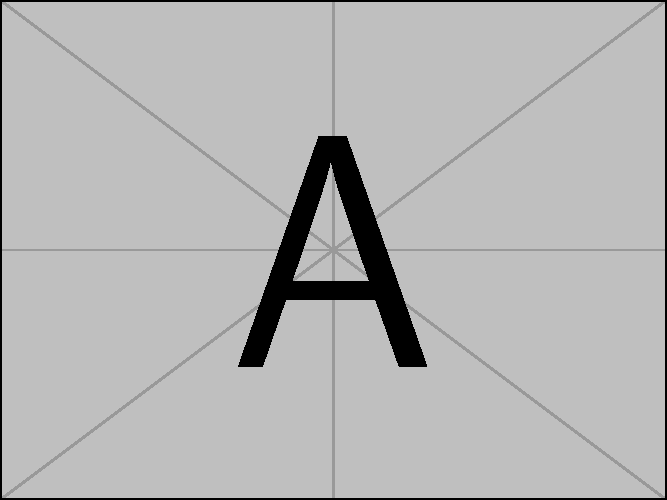
\includegraphics[width=0.5\linewidth]{example-image-a.pdf}
	\caption*{国外的期刊习惯将图表的标题和说明文字写成一段,需要改写为标题只含图表的名称,其他说明文字以注释方式写在图表下方,或者写在正文中。}
	\caption{示例图片标题}
	\label{fig:example}
\end{figure}

若图或表中有附注,采用英文小写字母顺序编号,附注写在图或表的下方。
国外的期刊习惯将图表的标题和说明文字写成一段,需要改写为标题只含图表的名称,其他说明文字以注释方式写在图表下方,或者写在正文中。

如果一个图由两个或两个以上分图组成时,各分图分别以 (a)、(b)、(c)...... 作为图序,并须有分图题。
推荐使用 \pkg{subcaption} 宏包来处理, 比如图~\ref{fig:subfig-a} 和图~\ref{fig:subfig-b}。

\begin{figure}
	\centering
	\subcaptionbox{分图 A\label{fig:subfig-a}}
	{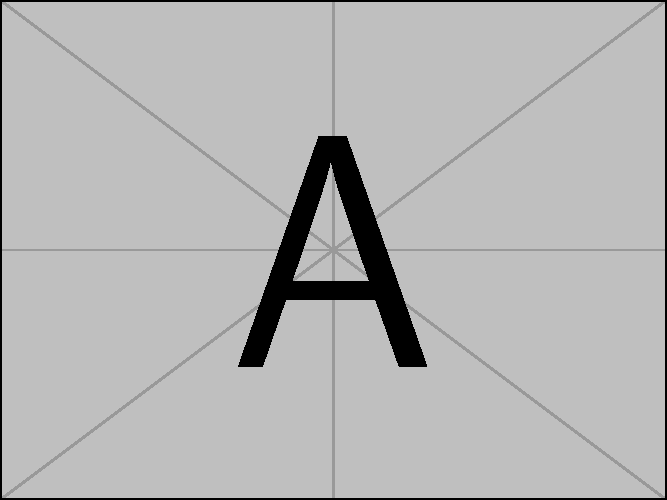
\includegraphics[width=0.35\linewidth]{example-image-a.pdf}}
	\subcaptionbox{分图 B\label{fig:subfig-b}}
	{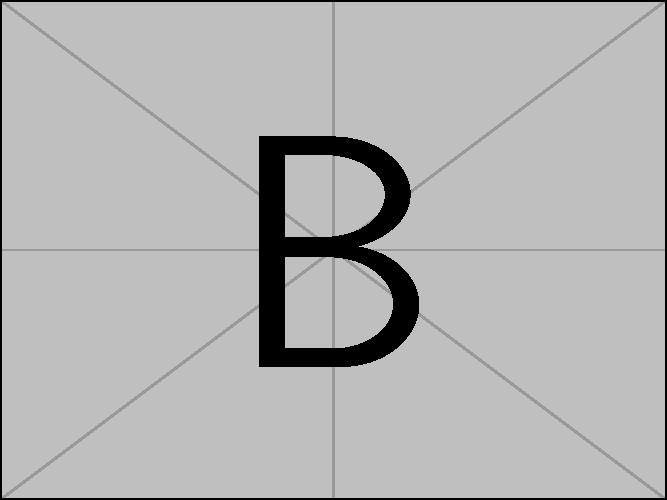
\includegraphics[width=0.35\linewidth]{example-image-b.pdf}}
	\caption{多个分图的示例}
	\label{fig:multi-image}
\end{figure}



\section{表格}

表应具有自明性。为使表格简洁易读,尽可能采用三线表,如表~\ref{tab:three-line}。
三条线可以使用 \pkg{booktabs} 宏包提供的命令生成。

\begin{table}
	\centering
	\caption{三线表示例}
	\begin{tabular}{ll}
		\toprule
		文件名          & 描述                         \\
		\midrule
		thuthesis.dtx   & 模板的源文件,包括文档和注释 \\
		thuthesis.cls   & 模板文件                     \\
		thuthesis-*.bst & BibTeX 参考文献表样式文件    \\
		\bottomrule
	\end{tabular}
	\label{tab:three-line}
\end{table}

表格如果有附注,尤其是需要在表格中进行标注时,可以使用 \pkg{threeparttable} 宏包。
研究生要求使用英文小写字母 a、b、c……顺序编号,本科生使用圈码 ①、②、③……编号。

\begin{table}
	\centering
	\begin{threeparttable}[c]
		\caption{带附注的表格示例}
		\label{tab:three-part-table}
		\begin{tabular}{ll}
			\toprule
			文件名                 & 描述                         \\
			\midrule
			thuthesis.dtx\tnote{a} & 模板的源文件,包括文档和注释 \\
			thuthesis.cls\tnote{b} & 模板文件                     \\
			thuthesis-*.bst        & BibTeX 参考文献表样式文件    \\
			\bottomrule
		\end{tabular}
		\begin{tablenotes}
			\item [a] 可以通过 xelatex 编译生成模板的使用说明文档;
			使用 xetex 编译 \file{thuthesis.ins} 时则会从 \file{.dtx} 中去除掉文档和注释,得到精简的 \file{.cls} 文件。
			\item [b] 更新模板时,一定要记得编译生成 \file{.cls} 文件,否则编译论文时载入的依然是旧版的模板。
		\end{tablenotes}
	\end{threeparttable}
\end{table}

如某个表需要转页接排,可以使用 \pkg{longtable} 宏包,需要在随后的各页上重复表的编号。
编号后跟表题(可省略)和“(续)”,置于表上方。续表均应重复表头。

\begin{longtable}{cccc}
	\caption{跨页长表格的表题} \\
	\toprule
	表头 1 & 表头 2 & 表头 3 & 表头 4 \\
	\midrule
	\endfirsthead
	\caption[]{跨页长表格的表题(续)} \\
	\toprule
	表头 1 & 表头 2 & 表头 3 & 表头 4 \\
	\midrule
	\endhead
	\bottomrule
	\endfoot
	Row 1  & & & \\
	Row 2  & & & \\
	Row 3  & & & \\
	Row 4  & & & \\
	Row 5  & & & \\
	Row 6  & & & \\
	Row 7  & & & \\
	Row 8  & & & \\
	Row 9  & & & \\
	Row 10 & & & \\
\end{longtable}



\section{算法}

算法环境可以使用 \pkg{algorithms} 或者 \pkg{algorithm2e} 宏包。

\renewcommand{\algorithmicrequire}{\textbf{输入:}\unskip}
\renewcommand{\algorithmicensure}{\textbf{输出:}\unskip}

\begin{algorithm}
	\caption{Calculate $y = x^n$}
	\label{alg1}
	\small
	\begin{algorithmic}
		\REQUIRE $n \geq 0$
		\ENSURE $y = x^n$
		
		\STATE $y \leftarrow 1$
		\STATE $X \leftarrow x$
		\STATE $N \leftarrow n$
		
		\WHILE{$N \neq 0$}
		\IF{$N$ is even}
		\STATE $X \leftarrow X \times X$
		\STATE $N \leftarrow N / 2$
		\ELSE[$N$ is odd]
		\STATE $y \leftarrow y \times X$
		\STATE $N \leftarrow N - 1$
		\ENDIF
		\ENDWHILE
	\end{algorithmic}
\end{algorithm}


模板支持 BibTeX 和 BibLaTeX 两种方式处理参考文献。
下文主要介绍 BibTeX 配合 \pkg{natbib} 宏包的主要使用方法。


\section{顺序编码制}

在顺序编码制下,默认的 \cs{cite} 命令同 \cs{citep} 一样,序号置于方括号中,
引文页码会放在括号外。
统一处引用的连续序号会自动用短横线连接。

\thusetup{
	cite-style = super,
}
\begin{tabular}{l@{\quad$\Rightarrow$\quad}l}
	\verb|\cite{zhangkun1994}|               & \cite{zhangkun1994}               \\
	\verb|\citet{zhangkun1994}|              & \citet{zhangkun1994}              \\
	\verb|\citep{zhangkun1994}|              & \citep{zhangkun1994}              \\
	\verb|\cite[42]{zhangkun1994}|           & \cite[42]{zhangkun1994}           \\
	\verb|\cite{zhangkun1994,zhukezhen1973}| & \cite{zhangkun1994,zhukezhen1973} \\
\end{tabular}


也可以取消上标格式,将数字序号作为文字的一部分。
建议全文统一使用相同的格式。

\thusetup{
	cite-style = inline,
}
\begin{tabular}{l@{\quad$\Rightarrow$\quad}l}
	\verb|\cite{zhangkun1994}|               & \cite{zhangkun1994}               \\
	\verb|\citet{zhangkun1994}|              & \citet{zhangkun1994}              \\
	\verb|\citep{zhangkun1994}|              & \citep{zhangkun1994}              \\
	\verb|\cite[42]{zhangkun1994}|           & \cite[42]{zhangkun1994}           \\
	\verb|\cite{zhangkun1994,zhukezhen1973}| & \cite{zhangkun1994,zhukezhen1973} \\
\end{tabular}



\section{著者-出版年制}

著者-出版年制下的 \cs{cite} 跟 \cs{citet} 一样。

\thusetup{
	cite-style = author-year,
}
\begin{tabular}{l@{\quad$\Rightarrow$\quad}l}
	\verb|\cite{zhangkun1994}|                & \cite{zhangkun1994}                \\
	\verb|\citet{zhangkun1994}|               & \citet{zhangkun1994}               \\
	\verb|\citep{zhangkun1994}|               & \citep{zhangkun1994}               \\
	\verb|\cite[42]{zhangkun1994}|            & \cite[42]{zhangkun1994}            \\
	\verb|\citep{zhangkun1994,zhukezhen1973}| & \citep{zhangkun1994,zhukezhen1973} \\
\end{tabular}

\vskip 2ex
\thusetup{
	cite-style = super,
}
注意,引文参考文献的每条都要在正文中标注
\cite{zhangkun1994,zhukezhen1973,dupont1974bone,zhengkaiqing1987,%
	jiangxizhou1980,jianduju1994,merkt1995rotational,mellinger1996laser,%
	bixon1996dynamics,mahui1995,carlson1981two,taylor1983scanning,%
	taylor1981study,shimizu1983laser,atkinson1982experimental,%
	kusch1975perturbations,guangxi1993,huosini1989guwu,wangfuzhi1865songlun,%
	zhaoyaodong1998xinshidai,biaozhunhua2002tushu,chubanzhuanye2004,%
	who1970factors,peebles2001probability,baishunong1998zhiwu,%
	weinstein1974pathogenic,hanjiren1985lun,dizhi1936dizhi,%
	tushuguan1957tushuguanxue,aaas1883science,fugang2000fengsha,%
	xiaoyu2001chubanye,oclc2000about,scitor2000project%
}。


\section{数学符号}

中文论文的数学符号默认遵循 GB/T 3102.11—1993《物理科学和技术中使用的数学符号》
\footnote{原 GB 3102.11—1993,自 2017 年 3 月 23 日起,该标准转为推荐性标准。}。
该标准参照采纳 ISO 31-11:1992 \footnote{目前已更新为 ISO 80000-2:2019。},
但是与 \TeX{} 默认的美国数学学会(AMS)的符号习惯有所区别。
具体地来说主要有以下差异:
\begin{enumerate}
	\item 大写希腊字母默认为斜体,如
	\begin{equation*}
		\Gamma \Delta \Theta \Lambda \Xi \Pi \Sigma \Upsilon \Phi \Psi \Omega.
	\end{equation*}
	注意有限增量符号 $\increment$ 固定使用正体,模板提供了 \cs{increment} 命令。
	\item 小于等于号和大于等于号使用倾斜的字形 $\le$、$\ge$。
	\item 积分号使用正体,比如 $\int$、$\oint$。
	\item 行间公式积分号的上下限位于积分号的上下两端,比如
	\begin{equation*}
		\int_a^b f(x) \dif x.
	\end{equation*}
	行内公式为了版面的美观,统一居右侧,如 $\int_a^b f(x) \dif x$ 。
	\item
	偏微分符号 $\partial$ 使用正体。
	\item
	省略号 \cs{dots} 按照中文的习惯固定居中,比如
	\begin{equation*}
		1, 2, \dots, n \quad 1 + 2 + \dots + n.
	\end{equation*}
	\item
	实部 $\Re$ 和虚部 $\Im$ 的字体使用罗马体。
\end{enumerate}

以上数学符号样式的差异可以在模板中统一设置。
另外国标还有一些与 AMS 不同的符号使用习惯,需要用户在写作时进行处理:
\begin{enumerate}
	\item 数学常数和特殊函数名用正体,如
	\begin{equation*}
		\uppi = 3.14\dots; \quad
		\symup{i}^2 = -1; \quad
		\symup{e} = \lim_{n \to \infty} \left( 1 + \frac{1}{n} \right)^n.
	\end{equation*}
	\item 微分号使用正体,比如 $\dif y / \dif x$。
	\item 向量、矩阵和张量用粗斜体(\cs{symbf}),如 $\symbf{x}$、$\symbf{\Sigma}$、$\symbfsf{T}$。
	\item 自然对数用 $\ln x$ 不用 $\log x$。
\end{enumerate}


英文论文的数学符号使用 \TeX{} 默认的样式。
如果有必要,也可以通过设置 \verb|math-style| 选择数学符号样式。

关于量和单位推荐使用
\href{http://mirrors.ctan.org/macros/latex/contrib/siunitx/siunitx.pdf}{\pkg{siunitx}}
宏包,
可以方便地处理希腊字母以及数字与单位之间的空白,
比如:
\SI{6.4e6}{m},
\SI{9}{\micro\meter},
\si{kg.m.s^{-1}},
\SIrange{10}{20}{\degreeCelsius}。

\section{数学公式}

数学公式可以使用 \env{equation} 和 \env{equation*} 环境。
注意数学公式的引用应前后带括号,建议使用 \cs{eqref} 命令,比如式\eqref{eq:example}。
\begin{equation}
	\frac{1}{2 \uppi \symup{i}} \int_\gamma f = \sum_{k=1}^m n(\gamma; a_k) \mathscr{R}(f; a_k)
	\label{eq:example}
\end{equation}
注意公式编号的引用应含有圆括号,可以使用 \cs{eqref} 命令。

多行公式尽可能在“=”处对齐,推荐使用 \env{align} 环境。
\begin{align}
	a & = b + c + d + e \\
	& = f + g
\end{align}



\section{数学定理}

定理环境的格式可以使用 \pkg{amsthm} 或者 \pkg{ntheorem} 宏包配置。
用户在导言区载入这两者之一后,模板会自动配置 \env{thoerem}、\env{proof} 等环境。

\begin{theorem}[Lindeberg--Lévy 中心极限定理]
	设随机变量 $X_1, X_2, \dots, X_n$ 独立同分布, 且具有期望 $\mu$ 和有限的方差 $\sigma^2 \ne 0$,
	记 $\bar{X}_n = \frac{1}{n} \sum_{i+1}^n X_i$,则
	\begin{equation}
		\lim_{n \to \infty} P \left(\frac{\sqrt{n} \left( \bar{X}_n - \mu \right)}{\sigma} \le z \right) = \Phi(z),
	\end{equation}
	其中 $\Phi(z)$ 是标准正态分布的分布函数。
\end{theorem}
\begin{proof}
	Trivial.
\end{proof}

同时模板还提供了 \env{assumption}、\env{definition}、\env{proposition}、
\env{lemma}、\env{theorem}、\env{axiom}、\env{corollary}、\env{exercise}、
\env{example}、\env{remar}、\env{problem}、\env{conjecture} 这些相关的环境。

\fi